
\section{Preliminary Assessment of \iris}
\label{sec:assessment}

\subsection{Experimental Settings}
\label{sec:method}
The \emph{goal} of the study is to provide a preliminary assessment of the performance of the proposed framework, with the \emph{purpose} of understanding its potential usefulness for the data extraction stage of machine learning approaches. More specifically, we seek to understand computational time, which heavily depends on the structure and dimension of the analyzed repositories. Hence, we pose the following research question:

\begin{center}
	\begin{examplebox}
		\textbf{RQ$_1$.} \emph{To what extent can \iris improve the computational time with respect to a single-threaded baseline?}	
	\end{examplebox}
\end{center}

\textbf{Context selection.} The \emph{context} of the study is composed of the version history of the systems reported in Table \ref{tab:systems}. The selection process of those repositories is driven by their amount of commits available on the master branch (or more specifically, the branch which HEAD is pointing to). We assume that repositories with the most commits also contain a lot of refactoring operations. Additionally, projects are selected by their popularity and active contribution of developers. \ref{tab:systems} shows auxiliary metrics to get a better understanding about the shape of the repository in terms of time and file dimension. Since the history is changing, we extracted information about the minimum and maximum amount of files as well as the mean number of files and the deviation. Time dimension is represented by the amount of commits available on the master branch.

\begin{table}[htbp]
\caption{Repository Dimensionality Metrics}
\label{tab:systems}
\begin{center}
\begin{tabular}{|l|c|c|c|c|}
\hline
&\multicolumn{3}{c|}{Files}&\\
\hline
\textbf{Repository}&\textbf{Min}&\textbf{Max}&\textbf{Mean}&\textbf{Commit}\\
\hline
google/guava& 4 & 1862 & 1589.4 & 5295\\
\hline
apache/mahout& 5 & 1245 & 4145.1 & 4417\\
\hline
reactivex/rxjava& 65 & 3173 & 4878.9 & 5755\\
\hline
apache/parquet-mr & 2 & 802 & 2013.4 & 2188\\
\hline
apache/commons-io & 21 & 317 & 2107.9 & 2384\\
\hline
\end{tabular}
\end{center}
\end{table}

\textbf{Evaluation methodology.} For the runtime evaluation, a Spark cluster with a maximum amount of eight worker nodes is used. To observe the impact of distribution, each project is run with a different number of worker nodes \emph{w}. Since no tool currently is capable of running a whole pipeline, the setting with only one worker node (\emph{w = 1}) is used as an reference implementation for no parallelization. Each worker only makes use of one core, therefore the parallelization focuses on the distribution within the cluster. The jobs are executed with \emph{w = 1}, \emph{w = 2}, \emph{w = 4} and \emph{w = 8}. To provide a better insight in the measured runtimes, we also collected additional metrics about the each step (refactoring mining and metric calculation) and the amount of output data generated by each repository. Additionally, we cloned and prepared the repositories before each run to avoid the bias of the network connection.\\
\textbf{Evaluation hardware setting.} The evaluation is done on a single server running multiple virtual machines, each representing a Spark node. The machine has four Intel Xeon E-7 4850 deca-core CPUs and 64GB of memory. Based on this machine, each job is executed with a limit of 7GB of memory to keep space for the master node, the virtual machine and the Java virtual machine overheads.

\subsection{Analysis of the results}
Figure \ref{fig:relativeruntime} shows the relative runtime per each repository and by increasing the number of worker nodes in the cluster as described before. All projects are benefitting from the parallelization approach, especially when between one and four worker nodes. When using eight worker nodes, the impact is less. The Apache Mahout project is the only one that gets even worse.

\begin{figure}[h]
    \centering
    \caption{Relative runtime per project and worker w}
    \label{fig:relativeruntime}
    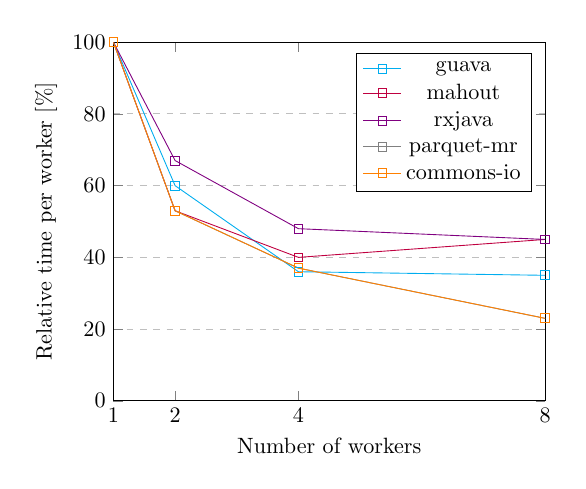
\begin{tikzpicture}[scale=0.8]
\begin{axis}[
    xlabel={Number of workers},
    ylabel={Relative time per worker [\%]},
    xmin=1, xmax=8,
    ymin=0, ymax=100,
    xtick={1,2,4,8},
    ytick={0,20,40,60,80,100},
    legend pos=north east,
    ymajorgrids=true,
    grid style=dashed,
]

\addplot[
    color=cyan,
    mark=square,
    ]
    coordinates {
    (1, 100)(2, 60)(4,36)(8,35)
    };
    \addlegendentry{guava}
    
\addplot[
    color=purple,
    mark=square,
    ]
    coordinates {
    (1, 100)(2, 53)(4,40)(8,45)
    };
    \addlegendentry{mahout}
\addplot[
    color=violet,
    mark=square,
    ]
    coordinates {
    (1, 100)(2, 67)(4,48)(8,45)
    };
    \addlegendentry{rxjava}
\addplot[
    color=gray,
    mark=square,
    ]
    coordinates {
    (1, 100)(2, 53)(4,37)(8,23)
    };
    \addlegendentry{parquet-mr}
\addplot[
    color=orange,
    mark=square,
    ]
    coordinates {
    (1, 100)(2, 53)(4,37)(8,23)
    };
    \addlegendentry{commons-io}
\end{axis}
\end{tikzpicture}
\end{figure}

Figure \ref{fig:taskratio} visualizes the consumption of computation time between task 1 and task 2 over all projects. We decide to use the mean value over all \emph{w}-values since the ratio is more or less the same for all \emph{w}. Task 2 is in the most cases more dominant in computation time consumption than task 1.

\begin{figure}[h]
    \centering
    \caption{Mean ratio between task 1 and task 2 for each project}
    \label{fig:taskratio}
    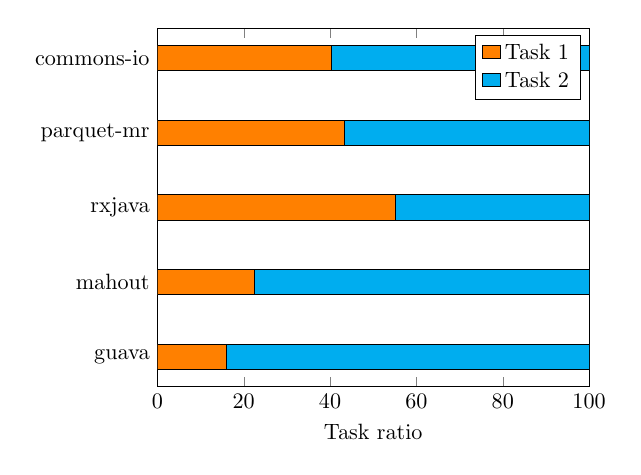
\begin{tikzpicture}[scale=0.8]
  \begin{axis}[
    xbar stacked, xmin=0, xmax=100,
    xlabel={Task ratio},
    bar width=4mm,
    symbolic y coords={guava,mahout,rxjava,parquet-mr, commons-io},
    ytick=data
  ]
\addplot [fill=orange] coordinates {
    (16.07,guava)
    (22.4,mahout)
    (55.06,rxjava)
    (43.38,parquet-mr)
    (40.25,commons-io)};
\addplot [fill=cyan] coordinates {
    (83.93,guava)
    (77.6,mahout)
    (44.94,rxjava)
    (56.62,parquet-mr)
    (69.05,commons-io)};
\legend{Task 1,Task 2}
\end{axis}
\end{tikzpicture}
\end{figure}

Table \ref{tab:detectedrefandmetrics} contains information about the amount of found refactoring operations and metrics. 

\begin{table}[ht]
\caption{Detected refactorings and metrics per project}
\label{tab:detectedrefandmetrics}
\begin{center}
\begin{tabular}{|l|c|c|c|c|}
\hline
\textbf{Repository}&\textbf{Refactoring operations}&\textbf{Metrics}\\
\hline
google/guava& 24732 & 18148\\
\hline
apache/mahout& 16471 & 20861\\
\hline
reactivex/rxjava& 41391 & 5654\\
\hline
apache/parquet-mr & 5459 & 5500\\
\hline
apache/commons-io & 3482 & 1517\\
\hline
\end{tabular}
\end{center}
\end{table}

We also discovered that in parallelized mode some worker nodes have a longer calculation time than others. Therefore, the variance is calculated for \emph{w = 8} and task 1 and 2 to get an impression about how much both tasks vary in their single runtime (table \ref{tab:variance}).

\begin{table}[ht]
\caption{$\sigma^2$-comparison between Task 1 and Task 2 for w = 8}
\label{tab:variance}
\begin{center}
\begin{tabular}{|l|c|c|c|c|}
\hline
\textbf{Repository}&  \textbf{Task 1}&\textbf{Task 2}\\
\hline
google/guava& 24.3 & 8.6\\
\hline
apache/mahout& 5.3 & 2.0\\
\hline
reactivex/rxjava& 73.0 & 66.9\\
\hline
apache/parquet-mr& 0.6 & 0.3\\
\hline
apache/commons-io& 0.4 & 0.5\\
\hline
\end{tabular}
\end{center}
\end{table}

Ultimately, we consider the throughput which is basically the number of outputs over the computation time needed to produce those output values. The throughput should result in an understandable visualization of the overhead introduced through parallelization. We slightly modified the throughput calculation showed below where \emph{wid} is the id of the worker available, \emph{r} is the amount of refactorings and m the amount of metrics.

\begin{equation*}
    throughput = \frac{\sum_{wid=1}{runtime(wid)}}{r+m}
\end{equation*}

Throughput is calculated by the accumulation of all single worker tasks. On a single node cluster this is just the maximum runtime. In parallelized mode, the time of each worker is accumulated, even when those workers are running concurrently and the effective time is shorter. How many items less can be calculated when using parallelization is presented in table \ref{fig:throughput}.

\begin{figure}[ht]
    \centering
    \caption{Throughput }
        \label{fig:throughput}
        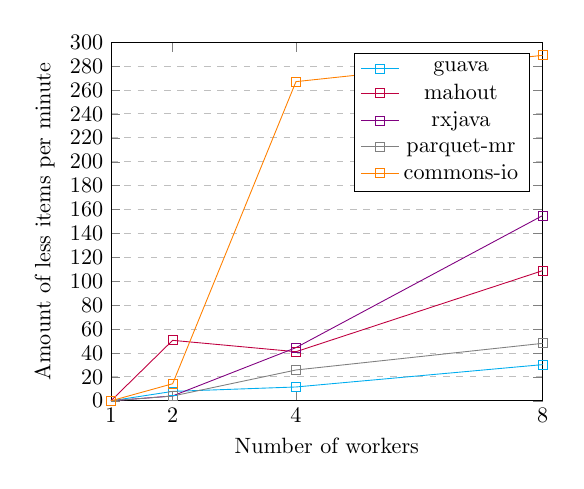
\begin{tikzpicture}[scale=0.8]
\begin{axis}[
    xlabel={Number of workers},
    ylabel={Amount of less items per minute},
    xmin=1, xmax=8,
    ymin=0, ymax=300,
    xtick={1,2,4,8},
    ytick={0,20,40,60,80,100,120,140,160,180,200,220,240,260,280,300},
    legend pos=north east,
    ymajorgrids=true,
    grid style=dashed,
]

\addplot[
    color=cyan,
    mark=square,
    ]
    coordinates {
    (1, 0)(2, 7.9)(4,11.6)(8,30.3)
    };
    \addlegendentry{guava}
    
\addplot[
    color=purple,
    mark=square,
    ]
    coordinates {
    (1, 0)(2, 50.6)(4,41.1)(8,108.9)
    };
    \addlegendentry{mahout}
\addplot[
    color=violet,
    mark=square,
    ]
    coordinates {
    (1, 0)(2, 4.1)(4,44.5)(8,155)
    };
    \addlegendentry{rxjava}
\addplot[
    color=gray,
    mark=square,
    ]
    coordinates {
    (1, 0)(2, 4)(4,25.8)(8,48.1)
    };
    \addlegendentry{parquet-mr}
\addplot[
    color=orange,
    mark=square,
    ]
    coordinates {
    (1, 0)(2, 14.3)(4,267)(8,289)
    };
    \addlegendentry{commons-io}
\end{axis}
\end{tikzpicture}
\end{figure}